\chapter{Implementation} \label{ch:implementation}

As described in Chapter \ref{ch:design} several design decisions were made to address the core functionality requirements. With Corda chosen as the private permissioned blockchain platform, an appropriate IAM solution was engineered as described in Section \ref{sec:iam-design}. Section \ref{sec:eduid-integration} goes through the high-level necessary technical steps for Swiss Educhain to integrate with SWITCH edu-ID. Section \ref{sec:implementation-code-structure} describes the parts of the codebase relevant to Swiss Educhain's IAM solution. Section \ref{sec:implementation-cordapp} demonstrates how the identity management part of Swiss Educhain is implemented in the CorDapp code. Lastly, Section \ref{sec:implementation-spring-boot} demonstrates the implementation details of the Spring Boot essential sub-components. High-level information and guidelines on how to install and configure the Swiss Educhain are provided in Appendix \ref{app:guidelines}.


\section{Integration with SWITCH edu-ID} \label{sec:eduid-integration}

As already analyzed in Section \ref{ssec:iam-solution} the chosen IAM solution is participation in the SWITCH federation and integration with SWITCH edu-ID. Swiss Educhain participates as a Service Provider (SP) and needs to implement certain technical integration steps as described in the next Sections.

\subsection{Shibboleth Installation and Configuration} \label{ssec:shib-implementation}

The Shibboleth Service Provider software needs to be installed to the server that hosts the Swiss Educhain service. The Swiss Educhain service is hosted on an Ubuntu Server provided by the Communications Systems Research Group (CSG) at the Department of Informatics. The service can be accessed at \url{https://educhain.csg.uzh.ch/app/}. Figure \ref{fig:aai-guides-sp} shows how the Shibboleth SP daemon integrates with Webservers.

\begin{figure}[H]
	\centering
	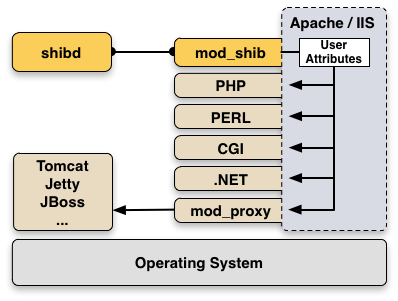
\includegraphics[width=0.5\textwidth]{figs/ch5/shib-sp}
	\caption{Shibboleth daemon integration \cite{aai-guides-sp}.}
	\label{fig:aai-guides-sp}
\end{figure}

The Shibboleth Service Provider consists of a daemon \texttt{shibd} running on all major operating systems and a web server module \texttt{mod\_shib} which is natively supported by the Apache HTTPD server.
The Service Provider can protect any web server content by enforcing user authentication \cite{aai-guides-sp}. Detailed step-by-step instructions for the installation and configuration of the Shibboleth Service Provider (SP) 3.0, as well as instructions on how to register an SP at the Resource Registry are provided by SWITCH \cite{shibboleth-installation}, \cite{shibboleth-configuration}.  

\subsection{HTTPS Configuration}

To provide integrity, security and confidentiality the Swiss Educhain service uses HTTPS traffic. This requires an SSL/TLS (Secure Sockets Layer, Transport Layer Security) Certificate by a trusted CA (Certificate Authority). Swiss Educhain uses \textbf{certbot} to create and renew automatically certificates signed by \textbf{Let's Encrypt} \cite{certbot-website}, \cite{lets-encrypt}. \\


\begin{lstlisting}[label=lst:apache-http-redirect, caption=Excerpt of the \texttt{apache2/sites-enabled/educhain.conf} file., language=apache]
RewriteEngine on
RewriteCond %{SERVER_NAME} =educhain.csg.uzh.ch
RewriteRule ^ https://%{SERVER_NAME}%{REQUEST_URI} [END,NE,R=permanent]
\end{lstlisting}

Once the certificate has been created, Apache is configured to redirect all \texttt{http} requests to \texttt{https}. Listing \ref{lst:apache-http-redirect} shows the \texttt{Rewrite} directives which are defined inside the port 80 \texttt{VirtualHost} configuration. \\


\begin{lstlisting}[label=lst:apache-https, caption=Excerpt of the \texttt{apache2/sites-enabled/educhain-le-ssl.conf} file., language=apache]
SSLEngine On
SSLProxyEngine On
SSLCertificateFile /etc/letsencrypt/live/example.com/fullchain.pem
SSLCertificateKeyFile /etc/letsencrypt/live/example.com/privkey.pem
Include /etc/letsencrypt/options-ssl-apache.conf
\end{lstlisting}


In Listing \ref{lst:apache-https} Apache is configured to turn on the SSL engine, the absolute paths are set for the generated certificate and private key, and the \texttt{options-ssl-apache.conf} file is imported from the \texttt{/etc/letsencrypt/} directory. This configuration file allows for further customization of the SSL protocol, the ciphersuite and enabling or disabling compression amongst other options. \\
To ensure that communication is secure between Apache and Spring Boot, SSL needs to be configured for the AJP Connector as seen in Figure \ref{fig:arch-educhain} and explained in detail at Section \ref{ssec:ajp-implementation}. As mentioned in the guidelines provided in Appendix \ref{app:guidelines}, a PKCS12 (Public-Key Cryptography Standards 12) certificate needs to be generated based on the valid SSL certificate, instructions on how to create it are given in \cite{java-certificate}. The variables in Listing \ref{lst:ssl-variables} need to be set in the \texttt{application.properties} file of the \texttt{clients} module, so Spring Boot is able to use the keystore. \\

\begin{lstlisting}[label=lst:ssl-variables, caption=Spring Boot embedded server SSL properties., language=Kotlin]
server.ssl.key-store = /path/keystore.p12
server.ssl.key-store-password = notapassword
server.ssl.keyStoreType = PKCS12
server.ssl.key-alias = mytomcat
\end{lstlisting}


\subsection{Shibboleth Access Control} \label{ssec:apache-httpd-implementation}

When configuration is in place for all the components to communicate securely and Swiss Educhain has been registered and integrated as a Service Provider, access controls can be defined through Shibboleth. \\

%\begin{lstlisting}[label=lst:apache-shib-handler, caption=Handler for \texttt{Shibboleth.sso} location., language=apache]
%<Location /Shibboleth.sso>
%	SetHandler shib
%</Location>
%\end{lstlisting}

\begin{lstlisting}[label=lst:apache-shib-access-control, caption=Access control for \texttt{/app/} location based on Shibboleth attributes., language=apache]
<Location /app/>
  AuthType shibboleth
  ShibRequestSetting requireSession true
  ShibUseEnvironment On
  <RequireAll>
	Require shib-attr swissEduIDLinkedAffiliation ~ .*@.*
	Require shib-attr matriculationNumber ~ .*
  </RequireAll>
</Location>
\end{lstlisting}

The configuration in Listing \ref{lst:apache-shib-access-control}, stored in \texttt{apache2.conf}, sets the following requirements to allow access to the protected resource in \url{https://educhain.csg.uzh.ch/app/}: 

\begin{itemize}
	\itemsep0em
	\item A valid active Shibboleth session.
	\item Shibboleth should use the environment to disclose attributes instead of the headers. This affects the way Spring Boot retrieves the already disclosed attributes which reside in Apache. More details on this process are provided in Section \ref{ssec:ajp-implementation}.
	\item Each user should have at least one linked affiliation with an Organization \textbf{and} the matriculation number should be present. If only one of the two is true, then access is denied.
\end{itemize}

The above access control is an implementation of the Service-level authorization as defined in Section \ref{ssec:educhain-authorization-policy}. More examples of Shibboleth Service Provider access control rules are provided in \cite{shib-access-control-rules}.


\subsection{Attributes} \label{impl-attributes}

As already described in detail in Section \ref{ssec:iam-solution} several attributes are necessary for Swiss Educhain to function. Swiss Educhain states in the Resource Description in the SWITCHaai Resource Registry (RR) which attributes are required and which are desired. Required are the core attributes which are available from all Organizations and desired are other attributes. If an attribute is neither required nor desired by the SP, then it will not be disclosed at all. Swiss Educhain attributes:

\begin{description}
	\itemsep0em
	\item\textbf{commonName (cn)} - core, required.
	\item\textbf{mail} - core, required.
	\item\textbf{persistentID} - core, required.
	\item\textbf{matriculationNumber} - other, desired.
	\item\textbf{swissEduIDLinkedAffiliation} - other, desired.
\end{description}

Shibboleth checks only if \texttt{matriculationNumber} and \texttt{swissEduLinkedAffiliation} exist and have the proper value, because these attributes are not guaranteed to be present in a user's account. The Spring Boot module can request the value of one or more attributes by calling the \texttt{request.getAttribute()} method and specifying the attribute to be fetched by \texttt{name}. An example of all the attributes disclosed in a session are shown in Figure \ref{fig:sso-attributes}. 

\begin{figure}[H]
	\centering
	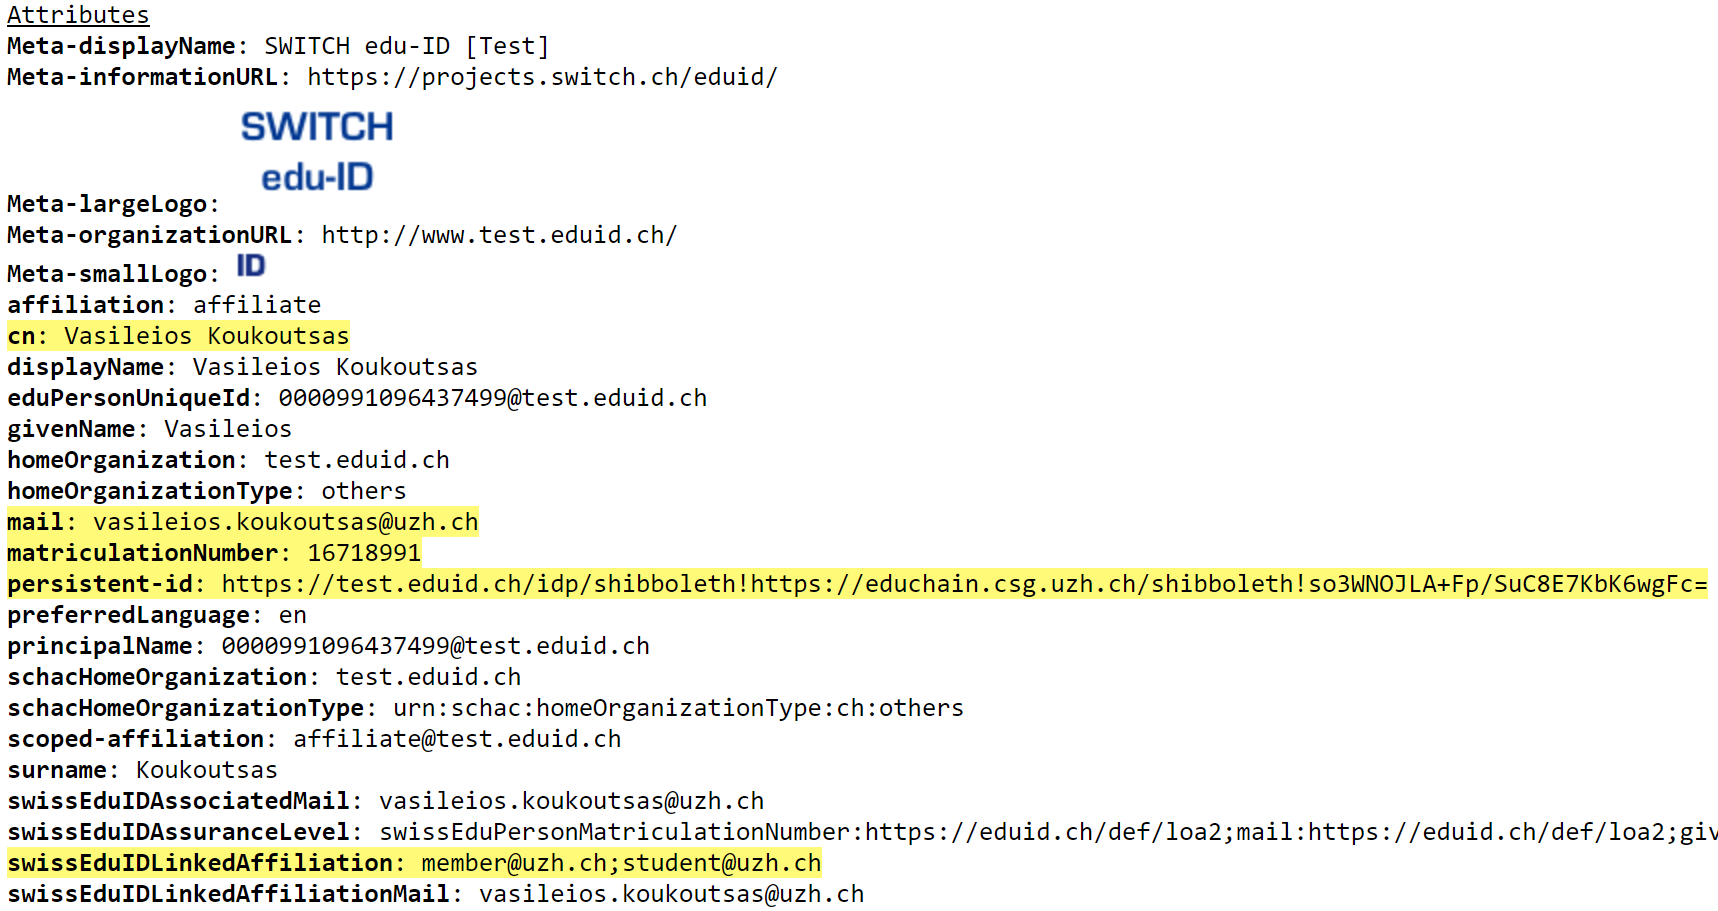
\includegraphics[width=0.75\textwidth]{figs/ch5/sso-session-attributes}
	\caption{SSO session attributes disclosed to Swiss Educhain.}
	\label{fig:sso-attributes}
\end{figure}



\section{Code Structure} \label{sec:implementation-code-structure}

The Swiss Educhain service in its core is developed as a CorDapp (Corda Decentralized Application). The codebase has been based on the CorDapp Kotlin template \cite{kotlin-cordapp-template} and was expanded to meet the MVP functionality needs both for the identity management and the verification process. 

The main code modules of the service are:
\begin{description}
	\itemsep0em 
	\item\textbf{clients} \hfill \\
	This is the \texttt{Spring Boot} component and it contains: 
	\begin{description}
		\itemsep0em
		\item - the web \texttt{frontend} code, which is written in \texttt{HTML} and \texttt{AngularJS},
		\item - the embedded \texttt{Tomcat Server} (with the attached \texttt{AJP} connector),
		\item - the \texttt{Controller} exposing \texttt{RESTful} endpoints to interact with the \texttt{CorDapp}.
	\end{description} 
	\item\textbf{contracts} \hfill \\
	This is a \texttt{CorDapp} component and contains the \texttt{Contracts} and \texttt{States} definitions. 

	\item\textbf{verification\_frontend} \hfill \\ 
	Contains the verification frontend files, it is written in plain \texttt{HTML} and \texttt{JavaScript}.
	\item\textbf{workflows} \hfill \\
	This module contains the majority of the \texttt{CorDapp} functionality:
	\begin{description}
		\itemsep0em
		\item - the  \textbf{flows} for \texttt{Account} and \texttt{Diploma} functionality,  
		\item - \texttt{RPC} startable \textbf{queries} to retrieve data from the node \texttt{Vault},
		\item - the \texttt{Identity} and \texttt{Ethereum} node \textbf{services},
		\item - the \texttt{Solidity} \textbf{smart contract}.
	\end{description} 
\end{description}

The CorDapp consists of two code modules, namely \texttt{contracts} and \texttt{workflows}. There are two reasons behind this decision. Firstly, the contract JAR is attached to a transaction and independent upgrades, so producing it separately reduces its size significantly. Secondly, contracts have \texttt{constraints} and upgrading is complex, therefore decoupling contract code from flow code allows flows to be upgraded independently. \\
A high-level file structure of the code is presented in Appendix \ref{app:code-structure}, and the complete Swiss Educhain source code can be found in the contents of the accompanying CD. In the following Sections, only the functionality strictly related to identity and access management is analyzed, a detailed analysis on the functionality related to the verification process is provided in Simon M{\"u}ller's work \cite{mueller20}.


\section{CorDapp} \label{sec:implementation-cordapp}

The application logic and core functionality of the Swiss Educhain is implemented as a CorDapp. Same as any other CorDapp, it needs to have a few building blocks to be complete such as states, contracts, flows and (optionally) services.   

\subsection{Swiss Educhain Application Accounts}

As previously explained in Section \ref{ssec:iam-solution} to create an Educhain application account some fields are retrieved through attributes, some fields are populated inside the CorDapp and a one-to-one mapping to Corda technical accounts must be defined. Figure \ref{fig:identity-mapping} demonstrates the different fields and the exact data flow. To provide debugging information in the web frontend the sections of \texttt{Educhain Accounts} and \texttt{Corda Accounts} are displayed as shown in Figure \ref{fig:frontend-accounts}. 

\begin{figure}[H]
	\centering
	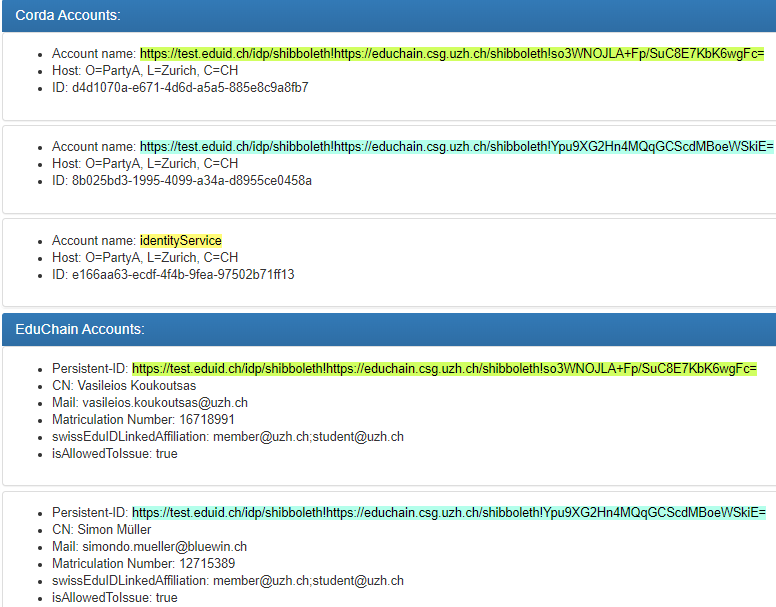
\includegraphics[width=0.6\textwidth]{figs/ch5/frontend-accounts-cropped}
	\caption{Educhain and Corda accounts frontend sections.}
	\label{fig:frontend-accounts}
\end{figure}

\subsection{Corda Accounts \& Node Identity Service}

As analyzed in Section \ref{ssec:corda-accounts} the Corda Accounts library offers the possibility to create technical Corda accounts with only three fields:
\begin{description}
	\itemsep0em
	\item\textbf{name} - can be set during the account creation (type \texttt{String}),
	\item\textbf{host} - is of type \texttt{Party} and is the identity of the node hosting the account,
	\item\textbf{identifier} - is a UUID (Universally Unique Identifier) value automatically generated of type \texttt{UniqueIdentifier}.
\end{description}

To create new accounts the \texttt{createAccount(name: String)} function is used which is defined in the \texttt{KeyManagementBackedAccountService} class \cite{corda-accounts-library}. Listing \ref{lst:corda-account} shows the Corda account state and creation function. After a Corda account has been created it can no longer be updated. The Corda accounts need to be leveraged from the application to create any custom accounts lifecycle or identity and access management solutions. \\

\begin{lstlisting}[label=lst:corda-account, caption=Corda \texttt{AccountInfo} state and \texttt{createAccount} function., language=Kotlin]
@BelongsToContract(AccountInfoContract::class)
data class AccountInfo(
  val name: String,
  val host: Party,
  val identifier: UniqueIdentifier
)
@Suspendable
override fun createAccount(name: String): CordaFuture<StateAndRef<AccountInfo>> {
  return flowAwareStartFlow(CreateAccount(name))
}
\end{lstlisting}

To facilitate a standardized and easily accessible way to create Corda accounts an identity service was created. Corda services run on a single node and offer functionality inside the node, they are initialized automatically when the node boots up, and they can only be called from within a flow or from another service through the \texttt{serviceHub} interface \cite{corda-services-101}. \\

\begin{lstlisting}[label=lst:identity-service, caption=Educhain Identity Service., language=Kotlin]
@CordaService
class EduChainIdentityService(private val serviceHub: AppServiceHub): SingletonSerializeAsToken() {
 @Suspendable
 fun createIdentityServiceAccount() : StateAndRef<AccountInfo> {
  val name: String = "identityService"
  try { // Check if account already exists
   require(serviceHub
    .cordaService(KeyManagementBackedAccountService::class.java)
    .accountInfo(name).none
    {serviceHub.myInfo.legalIdentities.contains(it.state.data.host)})
  } catch (ex: Exception){
   println(ex.message)
   return serviceHub.cordaService(KeyManagementBackedAccountService::class.java).accountInfo(name).get(0)
  } // Creates and returns the identityService account
  return serviceHub.accountService.createAccount(name).toCompletableFuture().getOrThrow()	
 }
}
\end{lstlisting}

Listing \ref{lst:identity-service} shows the service definition and the only service method \texttt{createIdentityServiceAccount}. This method is used to create the hardcoded Corda identity service account if does not exist. The \texttt{identityService} account is in turn used by the \texttt{(Create|Update)EduChainAccountFlow} to create the Educhain accounts during the flow's execution.

\subsection{Educhain Account State}

The \texttt{EduchainAccountState} holds the information of a user's account. The account is created based on a user's unique identifier which is the \texttt{persistentID} attribute generated by edu-ID to enable Swiss Educhain to identify a user. The
code of this state can be seen in Listing \ref{lst:educhain-account-state}. \\

\begin{lstlisting}[label=lst:educhain-account-state, caption=Code of \texttt{EduChainAccountState}., language=Kotlin]
@BelongsToContract(EduChainAccountContract::class)
data class EduChainAccountState(val persistentID: String,
  val cn: String,
  val mail: String,
  val matriculationNumber: String,
  val swissEduIDLinkedAffiliation: String,
  val issuer: AnonymousParty,
  val recipient: AnonymousParty,
  val isAllowedToIssue:  Boolean) : ContractState {
  override val participants get() = listOf(issuer, recipient)
}
\end{lstlisting}

The annotation in Line 1 signals that any modification of the \texttt{EduChainAccountState} by a flow must obey the rules defined in the \texttt{EduChainAccountContract}. The contract's rules and code is provided in Listing \ref{lst:educhain-account-contract}. The first five attributes disclosed by SWITCH edu-ID have been described in Section \ref{ssec:iam-solution}. A description for the fields that are generated by the CorDapp is given:

\begin{description}
	\itemsep0em
	\item\textbf{issuer} - the Corda account of the issuer of the Educhain account, of type \texttt{AnonymousParty} is a public key representation of the actual account.
	\item\textbf{recipient} - the Corda account of the recipient of the Educhain account, of type \texttt{AnonymousParty} is a public key representation of the actual account.
	\item\textbf{isAllowedToIssue} - determines if a user is an \texttt{Issuer} or not, it is generated in the \texttt{(Create|Update)EduChainAccountFlow}. It is always checked for validity by the \texttt{load-account} endpoint during each new session or webpage refresh.
\end{description}

\subsection{Educhain Account Contract} \label{ssec:educhain-account-contract}

The \texttt{EduChainAccountContract} is used by the \texttt{EduChainAccountState} and defines the possible actions that can modify an \texttt{EduChainAccountState}. The contract defines two possible commands \texttt{Create} and \texttt{Update}, which is derived from the high-level solution design that only allows for accounts to be created or updated. Currently, Educhain account deletion is not implemented to ensure there is transparency, traceability and verifiability of actions in the diploma issuance and verification process. \\

\begin{lstlisting}[label=lst:educhain-account-contract, caption=Code of the \texttt{EduChainAccountContract}., language=Kotlin]
class EduChainAccountContract : Contract {
 interface Commands : CommandData {
  class Create : TypeOnlyCommandData(), Commands
  class Update : TypeOnlyCommandData(), Commands
 }
 @Throws(IllegalArgumentException::class)
 override fun verify(tx: LedgerTransaction) {
  val command = tx.commands.requireSingleCommand<Commands>()
  val output = tx.outputsOfType<EduChainAccountState>().single()
  
  when (command.value) {
   is Commands.Create -> requireThat {
    "No inputs should be consumed when creating an EduChain account." using (tx.inputs.isEmpty())
    "Only one output state should be created when creating an EduChain account." using (tx.outputs.size == 1)
    val eduChainAccount = tx.outputStates.single() as EduChainAccountState
    "The account creator and account owner cannot have the same identity." using
     (output.participants[0] != output.participants[1])
    "Only account creator and account owner may sign the account create transaction." using
     (command.signers.toSet() == output.participants.map { it.owningKey }.toSet())
   }
   is Commands.Update -> requireThat {
     //Same as Create but allows one input state.
   }
  }
 }
}
\end{lstlisting}

There are four rules defined by the contract for the \texttt{Create} command as seen in Listing \ref{lst:educhain-account-contract}:

\begin{description}
	\itemsep0em
	\item - No inputs should be consumed when creating an Educhain account.
	\item - Only one output state should be created when creating an Educhain account.
	\item - The account creator and account owner cannot have the same identity.
	\item - Only account creator and account owner may sign account create transaction.	
\end{description}

The same rules apply to the \texttt{Update} command with the only difference being one input state is expected, which will be consumed and marked as historic, to produce one output (updated) state.


\subsection{Educhain Account Flows}

Corda flows are the mechanism that encapsulates the core business logic of a CorDapp. Simon M{\"u}ller in \cite{mueller20} provides an excellent skeleton of the Swiss Educhain flows in the form of pseudo-code, including a list of the main flow functionality. The pseudo-code is provided in Listing \ref{lst:flow-pseudo}. \\

\begin{lstlisting}[label=lst:flow-pseudo, caption=Pseudo-code of a typical Corda flow \cite{mueller20}., language=Kotlin, basicstyle=\scriptsize\ttfamily, numberstyle=\scriptsize]
@InitiatingFlow
@StartableByRPC
class Flow(private val exampleName: String,
private val exampleId: UUID) : FlowLogic<ReturnObject>() {
 companion object {
  /* ProgressTracker steps are defined here
   * They can be used during flow execution to track progress. */
  object FIRST_STEP : ProgressTracker.Step("First step")
  object SECOND_STEP : ProgressTracker.Step("Second step")
  fun tracker() = ProgressTracker(
      FIRST_STEP,
      SECOND_STEP )
 }
 override val progressTracker = tracker()
 @Suspendable
 override fun call(): ReturnObject {
  progressTracker.currentStep = FIRST_STEP
  /* Business logic of the flow is contained here.
  *  - Checking requirements,
  *  - Choosing the notary,
  *  - Requesting the public keys for the accounts,
  *  - Creating the transaction (input, output, command, attachment),
  *  - Gathering the signatures from all parties for the transaction,
  *  - Finalising the transaction. */
  progressTracker.currentStep = SECOND_STEP
  return ReturnObject()
 }
}
@InitiatedBy(Flow::class)
class FlowResponder(val counterPartySession: FlowSession) : FlowLogic<Unit>() {
 @Suspendable
 override fun call() {
 /* The response flow called as part of finalising a transaction.
  * Not every flow uses a response flow.
  * Code here typically involves verifying the transaction and recording the states. */ }
}
\end{lstlisting}

%The following flows relevant to identity and access management are described in detail:

\subsubsection{CreateEduChainAccountFlow}

\begin{lstlisting}[label=lst:educhain-create-account-flow, caption=Code snippet of the \texttt{CreateEduChainAccountFlow}., language=Kotlin, basicstyle=\scriptsize\ttfamily, numberstyle=\scriptsize]
// Retrieve the notary identity from the network map.
val notary = serviceHub.networkMapCache.notaryIdentities[0]
// Create or Fetch identityService account's UUID
val issuingAccountId: UUID = serviceHub.cordaService(EduChainIdentityService::class.java).createIdentityServiceAccount().state.data.identifier.id
// Retrieve the issuing/receiving accounts and their public keys
val issuingAccount = accountService.accountInfo(issuingAccountId)
?: throw FlowException("No account for ID $issuingAccountId found in vault.")
val receivingAccount = accountService.createAccount(name = persistentID).toCompletableFuture().getOrThrow()
val issuingAccountAnonParty = subFlow(RequestKeyForAccount(issuingAccount.state.data))
val receivingAccountAnonParty = subFlow(RequestKeyForAccount(receivingAccount.state.data))
// Check if an account has diplomas to be issued in the Waiting List
val diplomasIssuedFromWaitingList = mutableListOf<StateAndRef<DiplomaState>>()
val diplomaList = subFlow(CheckDiplomaWaitingListForMatriculationNumber(matriculationNumber))
for (diploma in diplomaList) {
 val diplomaIssuer = accountService.accountInfo(diploma.state.data.issuer.owningKey)
 if (diplomaIssuer?.state?.data?.identifier?.id == null) {
  // should not happen
  continue
 }
 val diplomaState=subFlow(IssueDiplomaToAccountFromWaitingList(diploma,
 diploma.state.data.diplomaAttachment,
 diploma.state.data.diplomaHash,
 diplomaIssuer.state.data.identifier.id,
 receivingAccount.state.data.identifier.id))
 diplomasIssuedFromWaitingList.add(diplomaState)
}
System.out.println("Diplomas issued from waiting list: ${diplomasIssuedFromWaitingList.size}")
// Determine if the account owner is allowed to issue
val issuersAffiliation=listOf<String>("faculty@uzh.ch","staff@uzh.ch")
val hardCodedIssuers=listOf<String>("16718991", "12715389", "12345678")
var isAllowedToIssue=false
for (it in issuersAffiliation) {
 if (swissEduIDLinkedAffiliation.contains(it)) {
  isAllowedToIssue = true }
}
if(hardCodedIssuers.contains(matriculationNumber)) isAllowedToIssue=true
// Create the transaction components.
val outputState = EduChainAccountState( persistentID, cn, mail, matriculationNumber, swissEduIDLinkedAffiliation, issuingAccountAnonParty, receivingAccountAnonParty, isAllowedToIssue)
val command = Command ( EduChainAccountContract.Commands.Create(), listOf(issuingAccountAnonParty.owningKey, receivingAccountAnonParty.owningKey))
// Create a transaction builder and add the transaction components
val txBuilder = TransactionBuilder(notary = notary)
 .addOutputState(outputState).addCommand(command)
// Sign the transaction.
val locallySignedTx = serviceHub.signInitialTransaction(
 txBuilder, listOfNotNull(issuingAccountAnonParty.owningKey, receivingAccountAnonParty.owningKey))
// Create a session with the other party.
val counterPartySession = initiateFlow(receivingAccount.state.data.host)
// Obtain the counterparty's signature and add to locally signed transaction
val receiverSignature = subFlow(CollectSignatureFlow(locallySignedTx, counterPartySession, receivingAccountAnonParty.owningKey))
val signedByCounterParty = locallySignedTx.withAdditionalSignatures(receiverSignature)
// Return fully signed transaction
return subFlow(FinalityFlow(signedByCounterParty, listOf(counterPartySession).filter
 { it.counterparty != ourIdentity }))
\end{lstlisting}

As shown in detail in Listing \ref{lst:educhain-create-account-flow} the following steps are executed in order with synchronous calls:

\begin{enumerate}
	\itemsep0em
	\item The notary's identity is retrieved from the network map.
	\item \texttt{identityService} account's UUID is created or fetched.
	\item Issuing and receiving accounts are retrieved and their public keys.
	\item It is checked if an account has diplomas to be issued in the waiting list.
	\item It is determined if the account owner should be allowed to issue.
	\item Transaction components are created.
	\item A transaction builder is created, and the transaction components are added.
	\item A session is created with the counterparty.
	\item Counterparty's signature is obtained and added to the locally signed transaction.
	\item Fully signed transaction is returned.
\end{enumerate}

\subsubsection{UpdateEduChainAccountFlow}

The \texttt{UpdateEduChainAccountFlow} flow is quite similar to the \texttt{CreateEduChainAccountFlow} flow, with a few distinct differences in the steps involved. The code implementation of \texttt{UpdateEduChainAccountFlow} is omitted as Listings \ref{lst:flow-pseudo} and \ref{lst:educhain-create-account-flow} provide a quite thorough walkthrough. The \texttt{UpdateEduChainAccountFlow} high-level steps are:

\begin{enumerate}
	\itemsep0em
	\item The notary's identity is retrieved from the network map.
	\item The Educhain account to be updated and its state are retrieved.
	\item \texttt{identityService} account's UUID is created or fetched.
	\item Issuing and receiving accounts are retrieved and their public keys.
	\item It is checked again if the account owner should be allowed to issue.
	\item Transaction components are created, including an input state to be consumed.
	\item A transaction builder is created and the transaction components are added.
	\item A session is created with the counterparty.
	\item Counterparty's signature is obtained and added to the locally signed transaction.
	\item Fully signed transaction is returned.
\end{enumerate}

\section{Spring Boot} \label{sec:implementation-spring-boot}

The Spring Boot component acts as a bridge between the end user and the CorDapp backend as shown in Figure \ref{fig:arch-educhain}. The AJP connector acts as a highway to serve the frontend and fetch attributes exposed using the Shibboleth environment. The frontend is a single webpage serving both \texttt{Issuers'} and \texttt{Recipients'} needs, and the controller exposes well-defined backend CorDapp functionality to the frontend via REST API (Application Programming Interface) endpoints. These three sub-components are analyzed further in this Section from the IAM perspective. 

\subsection{AJP Connector} \label{ssec:ajp-implementation}

The AJP connector is normally used in high-traffic scenarios to optimize performance between one or more webservers behind an Apache instance. In the Swiss Educhain service use case, it is preferred to provide a safer way to disclose the attributes through the environment instead of using http headers. It is defined based on custom properties and then added to the existing Tomcat connectors. Listing \ref{lst:ajp-connector} shows the properties defined and the method that creates a new \texttt{Context} and adds it to the Tomcat connectors. \\

\begin{lstlisting}[label=lst:ajp-connector, caption=Code of the \texttt{AJP Connector}., language=Kotlin]
@Bean
open fun servletContainer(): ServletWebServerFactory? {
 val tomcat: TomcatServletWebServerFactory = object : TomcatServletWebServerFactory() {
  override fun postProcessContext(context: Context) {
   val securityConstraint = SecurityConstraint()
   securityConstraint.userConstraint = "CONFIDENTIAL"
   val collection = SecurityCollection()
   collection.addPattern("/*")
   securityConstraint.addCollection(collection)
   context.addConstraint(securityConstraint)
  }
 }
 tomcat.addAdditionalTomcatConnectors(redirectConnector())
 return tomcat
}
var maxSize = 50000000
open fun redirectConnector(): Connector? {
  val connector = Connector("AJP/1.3")
  connector.scheme = "https"
  connector.port = 8009
  connector.secure = true
  connector.uriEncoding = "UTF-8"
  connector.allowTrace = false
  connector.maxPostSize = maxSize
  connector.maxSavePostSize = maxSize
  connector.redirectPort = 8443
  return connector
}
\end{lstlisting}

The connector uses the \texttt{port 8009} following common practice. The scheme is set to \texttt{https} and requires that the connection is \texttt{secure}. Furthermore, the \texttt{maximum POST} size is increased to allow for multiple attributes to be disclosed simultaneously. Apache configuration also needs to be updated to serve traffic through the \texttt{ajp} protocol. Listing \ref{lst:apache-ajp} shows the directive added to the \texttt{educhain-le-ssl.conf} file. It should be noted that the \texttt{ajp} protocol is used instead of the \texttt{http(s)} and that it is not possible to use both simultaneously. \\

\begin{lstlisting}[label=lst:apache-ajp, caption=Apache \texttt{AJP} proxy directive., language=apache]
ProxyPass /app/  ajp://localhost:8009/app/
\end{lstlisting}

\subsection{Controller}

The Controller is used as an intermediate to expose REST API endpoints to the web frontend and communicate with the CorDapp backend. The base path for all REST requests is \url{https://educhain.csg.uzh.ch/app/api/}. The main endpoints relevant to the identity and access management functionality are:

\subsubsection{load-account}
	\begin{itemize}
			\itemsep0em 
			\item Runs every time a new session is initiated. Checks if an Educhain account exists with the edu-ID user's \texttt{persistentID}, if it does not exist it is created, or if it exists but the attributes need to be updated they are updated. The endpoint calls \texttt{(Create|Update)EduChainAccountFlow}. 
			\item Method: \texttt{GET}
	\end{itemize}
	\subsubsection{my-account}
	\begin{itemize}
		\itemsep0em 
		\item Returns the user's \texttt{EduchainAccountState}.
		\item Method: \texttt{GET}
	\end{itemize}
	\subsubsection{edu-accounts}
		\begin{itemize}
			\itemsep0em 
			\item Returns a list of all the existing Educhain accounts' states.
			\item Method: \texttt{GET}
		\end{itemize}
	\subsubsection{own-accounts}
		\begin{itemize}
			\itemsep0em 
			\item Returns a list of all the existing Corda accounts.
			\item Method: \texttt{GET}
		\end{itemize}	
	\subsubsection{me}
		\begin{itemize}
			\itemsep0em 
			\item Returns the node's identity.
			\item Method: \texttt{GET}
		\end{itemize}

All account related API calls use the \texttt{GET} method, no account related fields need nor should be sent to the controller by the user or the frontend. Account information are fetched directly from edu-ID in the form of attributes for each session.
\subsection{Frontend Interface}

\emph{This is joint text with Simon M{\"u}ller \cite{mueller20}.}

The Swiss Educhain frontend is the main interactive part of Swiss Educhain. As soon as the user logs in via the edu-ID login screen, he is greeted by the Educhain frontend. It is a simple one-page website built with AngularJS \cite{angularjs} and styled with Bootstrap \cite{bootstrap}. \\
In the top left corner, the name of the node of the current connection is shown. Next to the node name the button 'Issue diploma' is placed. If the user that is logged in is not allowed to issue, it will be grayed out. The same applies to the 'Unsigned Diplomas' button next to it. The 'Logout' button in the top right logs out of the Swiss Educhain service and SWITCH edu-ID. Figure \ref{fig:educhain-frontend} shows the frontend with one issued diploma and two received diplomas.\\


\begin{figure}[H]
	\centering
	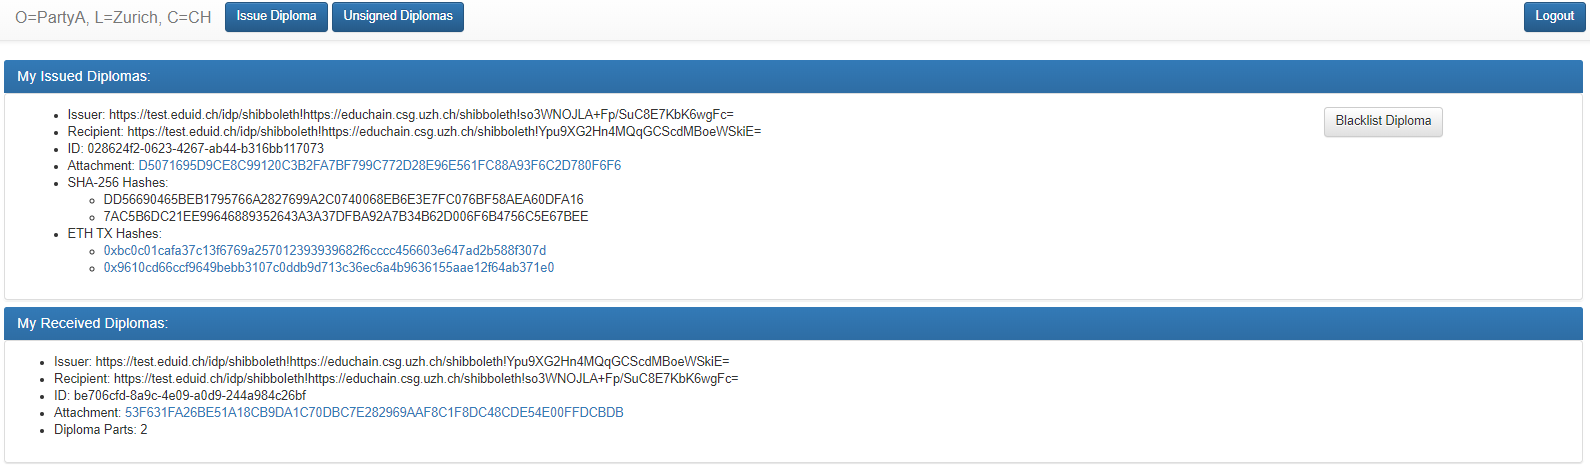
\includegraphics[width=\textwidth]{figs/ch5/frontend-issuer}
	\caption{Swiss Educhain frontend.}
	\label{fig:educhain-frontend}
\end{figure}

The view of the frontend is dedicated to showing information about the diplomas and the accounts available on the Corda node. The accounts are mainly shown for demonstration and debugging purposes. In a productive environment, only diplomas should be shown. The frontend has the following four main parts:

\begin{description}
	\itemsep0em
	\item\textbf{My Issued Diplomas} \hfill \\ 
	Shows a list of all issued diplomas by the logged-in account. This also includes diplomas for which the Ethereum transactions have not yet been signed. Selected information contained in the \texttt{DiplomaState} is shown for each entry in the list. Additionally, for every list entry that has been fully signed (i.e. broadcasted on the Ethereum network) there is also a button to blacklist the diploma, which will also exit the corresponding \texttt{DiplomaState}.
	
	\item\textbf{My Received Diplomas} \hfill \\ 
	Shows a list of all received diplomas by the logged-in account. Selected information contained in the \texttt{DiplomaState} is shown for each entry in the list.
	
	\item\textbf{Corda Accounts} \hfill \\ 
	Shows a list of all Corda accounts on the node. Information about each account is provided within the list entry. This is only for demonstration and debugging purposes.
	
	\item\textbf{Educhain Accounts} \hfill \\ 
	Shows a list of all Educhain accounts created on the node. Information about each account is provided within the list entry. This is only for demonstration and debugging purposes.
\end{description}

Clicking on the 'Issue Diploma' button will open a popup from where the \texttt{Issuer} can choose between a simple diploma issuance, extending an already existing diploma, issuing a batch of diplomas or broadcasting a transaction that was signed offline. The 'Unsigned Diplomas' button allows an \texttt{Issuer} to download a CSV (Comma-Separated values) file containing all the unsigned transactions that were generated by issuing a diploma air-gapped.

\emph{This ends the text jointly written with Simon M{\"u}ller \cite{mueller20}.}

